\documentclass[aps,pre,preprint,nofootinbib]{revtex4}

\usepackage{listings} 
\usepackage{graphicx}
\usepackage{epstopdf}
\usepackage{courier}
%\usepackage[scaled]{inconsolata}

%\usepackage{cite}

% type user-defined commands here

\begin{document}

\title{Erlang Term Storage Implementation}
\author{Kjell Winblad and Stavros Aronis}
\date{\today}


\begin{abstract}

This report describes in detail the implementation of Erlang Term Storage (ETS) tables as of version R15B02 of the Erlang/OTP distribution.
The main goal of this documentation attempt is to understand the scalability limitations that the current implementation imposes on applications that heavily use ETS tables.
With ETS tables often used to share data between processes in Erlang programs, it is important to have a scalable ETS implementation as data sharing is a common bottleneck in parallel applications.

In particular this report aims to become:
\begin{itemize}
\item a developer's guide to the current implementation of ETS tables;
\item a common base of knowledge for further discussion about possible improvements to the scalability of ETS within the context of the RELEASE project.
\end{itemize}

\end{abstract}

\maketitle

\section{Introduction to Erlang}\label{sec:erlang_intro}

Erlang is a garbage collected programming language especially designed to handle parallelism and fault-tolerance well.
An Erlang program consists of a number of processes.
Processes can be created by other processes.
An Erlang process consists of:
\begin{itemize}
 \item a mailbox for incoming messages from other processes (implemented as queue),
 \item the current execution stack,
 \item the process heap (containing data allocated by the process) and
 \item a process dictionary (a key-value map which can only be directly accessed from the owning process).
\end{itemize}
From the Erlang programmer's point of view, processes do not share any mutable data.
Processes communicate with each other by sending messages that will appear in the receiving process' mailbox.
The data in a message sent from one process to another, is in most cases copied from the heap of the sending process to the heap of the receiving process.
The exception, in the current Erlang/OTP distribution, is values of the binary data type.
Values of the binary data type are stored in a special data area and only the reference to the binary is copied when messages containing binaries are sent\footnote{Only the reference of the binary is copied when it is sent to another process in the same Erlang node, but the whole binary is copied if it is sent to a process in another Erlang node.}.
The allocation and deallocation of binaries is managed by reference counting.
The reasoning behind the special case for binaries, is that binaries are usually so large that it would be very expensive to do a full copy when sending them.

The copying can be expensive since the time and space required to do a copy depend on the size of the message.
However, the processes can be garbage collected independently when data is not shared by the processes.
The independent garbage collection can be important for the performance of parallel applications, since all other processes can continue unaffected while some are being garbage collected.
It is worth noting that the copying of messages is the implementation chosen for the current Erlang/OTP distribution but it may be changed in the future.
An alternative Erlang implementation that run on the Java Virtual Machine, called Erjang, just passes the messages' reference when messages are sent.
Thus, the Erjang implementation sends messages faster but can not garbage collect the processes independently.

\section{Introduction to Erlang Term Storage}

Erlang Term Storage (ETS) is a feature included in the Erlang/OTP runtime system.
It supports storage of Erlang tuples (also called \emph{objects} in this report) outside the processes' heaps.
ETS makes use of dedicated data structures called \emph{ETS tables} to store data.
The \emph{ETS tables} are mutable key-value maps.
ETS provides different table types with different properties, but they all share a common interface.

It is a well known fact that data that needs to be accessed and modified by several processes is a common bottleneck in parallel programs.
Therefore, it is important for Erlang programmers to have an efficient way of communicating data between processes.
In some programs the best way to communicate data between processes is to use Erlang's message system.
In other programs ETS can be used as a convenient and efficient way to accomplish data sharing. 
The program presented in Section~\ref{sec:benchmark} is an example of a program where ETS is useful.
An Erlang ETS table behaves as if a dedicated process served requests for insertions, lookups and other operations on a key-value dictionary.
However, since ETS is mostly implemented in the lower level programming language C, it is faster than what could be accomplished with a pure Erlang implementation.

The following are the major reasons why ETS can be more efficiently implemented in C than in Erlang\footnote{The major reason why C was chosen for implementing ETS and not any other lower level programming language is that Erlang/OTP runtime system is implemented in C.}:
\begin{itemize}
\item
Erlang does not have efficient support for working with mutable data.
The only way to handle mutable data inside an Erlang process is to use the Erlang process dictionary.
However, this is not very practical since the process dictionary was not designed to be used to implement advanced data structures.
\item 
The process garbage collector copy the process' data during collections.
Long-lived data are therefore copied many times during such passes. 
Storing this data in an ETS table which is not garbage collected can improve the efficiency of programs.
\end{itemize}

Erlang tuples that are inserted to an ETS table are copied from the heap of the process that is inserting the data to the table.
Erlang tuples that are retrieved from an ETS table are copied from the memory of the table to the retrieving process' heap.
Values of the binary data type are exceptions as they are when messages are sent between processes.
The reason why the whole tuple is copied and not just a reference to the tuple, is the same as the reason why messages are copied described in Section~\ref{sec:erlang_intro}.

ETS provides the most common table operations (insert, lookup and delete) as well as operations for searching for all tuples matching a specific criteria and for traversing the tuples in the table.

The Erlang database, Mnesia, gives the programmer an additional abstraction layer on top of ETS. 
Mnesia has support for:
\begin{itemize}
 \item persistent tables,
 \item synchronization of tables between Erlang nodes and
 \item transactions.
\end{itemize}

\section{Creating an ETS Table}

An ETS table can be accessed by either a \emph{table identifier} (TID) or an atom (in case of a \emph{named} table).
Table identifiers are created by calling the \verb|ets:new/2| BIF (Built-In Function).
The \verb|ets:new/2| BIF can also take a list of options that specify:

\begin{itemize}
\item
  The access level for the table which can be \verb|private|, \verb|protected| or \verb|public|.
  Only the creating process can read and write on \verb|private| tables, other processes may read but not write \verb|protected| tables and other processes can both read and write \verb|public| tables.
  More information about these options can be found at the Erlang documentation for ETS\footnote{http://www.erlang.org/doc/man/ets.html}.
\item
  Whether the table is a \verb|named_table|, in which case the atom provided as a table name can be used instead of the TID in table operations.
\item
  Whether the table type is \verb|set|, \verb|bag|, \verb|duplicate_bag|, or \verb|ordered_set|.
  The table types \verb|set|, \verb|bag| and \verb|duplicate_bag| are implemented as a linear hash table.
  In tables of the \verb|set| data type all inserted tuples need to have an unique queue.
  Whereas, in tables of the \verb|bag| data type there can be several tuples with the same key but all inserted tuples need to be unique.
  Finally, the \verb|duplicate_bag| allow several copies of the same tuple.
  The \verb|ordered_set| table type is implemented as AVL tree.
  When traversing the tuples in an \verb|ordered_set|, the tuples are guaranteed to come with the smallest keys first (All Erlang terms have a defined order.).
  See Section~\ref{sec:table_types} for information about the data structures used in the different table types.
\item
  Whether fine grained locking (\verb|write_concurrency|) and/or lock(s) optimized for frequent reads (\verb|read_concurrency|) should be used.
  The fine grained locking only affect the tables that are implement with the linear hash table.
  So specifying the \verb|write_concurrency| option together with the \verb|ordered_set| options does not have any effect.
  The effect of these options is described in more detail in Sections~\ref{sec:concurrency_options} and~\ref{sec:benchmark}.
\end{itemize}

ETS tables are ``owned'' by the creating process for as long as the creating process is alive, unless the ownership has been passed to another process with the \verb|ets:give_away/3| operation.
If the owner of an ETS table terminates the table will be deleted, unless the \verb|heir| option is set.
Developers can use the \verb|heir| option to specify a process that will inherit the table when the current owner terminates.
A process that is set as \verb|heir| will receive a message signaling the transfer of table ownership.

\section{Overview of Table Operations}

This section gives an overview of the most fundamental ETS table operations.
The Erlang documentation for ETS has a complete description of all table operations.
All operations are performed atomically, meaning that an operation would have the same effect if the process performing the operation was the only process.
However, there is no built-in support for performing a sequence of operations atomically.
Users that want to perform a sequence of operations atomically can use Mnesia or implement there own mechanism for ensuring atomicity.

\begin{description}
\item[lookup(Tab, Key) $\rightarrow$ {[Object]}]
  Returns a list of objects that have the given key.
\item[insert(Tab, ObjectOrObjects) $\rightarrow$ true]
  Insert the given object (or objects, if the parameter is a list of objects) to the table.
  It is common to use a programming pattern where first a lookup is made to check if a value with a certain key exists and then an insert is made to insert a new value if there was none before.
  This pattern can be problematic in a parallel application because another process might have inserted the value since the lookup.
  The Erlang/OTP developers saw this problem and added the \verb|insert_new| operator described below. 
\item[insert\_new(Tab, ObjectOrObjects) $\rightarrow$ boolean()]
  This operation will insert the given object or objects if no object with the same key as any of the object(s) exists.
  If a key already exists the operation will return \verb|false| and otherwise \verb|true|.
\item[delete(Tab, Key) $\rightarrow$ true]
  Deletes all objects with the given key from the table.
\item[first(Tab) $\rightarrow$ Key $|$ \texttt{end\_of\_table}]
  Returns the first key in the table.
  If the table is of the \verb|ordered_set| type, the first key in Erlang term order will be returned.
  If the table is of any other type, the first key according to the table's internal order will be returned.
  If the table is empty, \verb|end_of_table| will be returned.
\item[next(Tab, Key) $\rightarrow$ NextKey $|$ \texttt{end\_of\_table}]
  Given a key, this operation returns the next key appearing in the table.
  If the table is of the \verb|ordered_set| type, the next key in Erlang term order is returned.
  If the table is of any other type, the next key according to the table's internal order is returned.
  If there is no next key, \texttt{end\_of\_table} is returned.
\item[last(Tab) $\rightarrow$ Key $|$ \texttt{end\_of\_table}] Returns the last key in the table.
\end{description}

\section{Previous Work}

Scott Lystig Fritchie has suggested an ETS table implementation based on Judy-arrays~\cite{ScottEtsJudy}.
A Judy-array is a data structure similar to a trie but it uses compression techniques to waste less space and improve cache performance.
The performance of a Judy-array based implementation is experimentally compared to the AVL-tree (\verb|ordered_set|) and the linear hash table (\verb|set|, \verb|bag| and \verb|duplicate_bag|) implementations currently available.
For large table sizes the operations lookup, insert and update seem to be fastest with the Judy-array based implementation.
However, term deletion and table traversal seem to be slower in the Judy-array based implementation.
Fritchie does not give any suggestions on how to make a concurrent variant of the Judy-array based implementation.

Patrik Nyblom has suggested the addition of software transactional memory (STM) support for Erlang ETS tables~\cite{PatrikErlangTrans}.
Nyblom argued that STM support could be added to Erlang with only minor changes to the ETS implementation~\cite{PatrikErlangTrans}.
The suggested implementation would not effect the performance of ETS when the transactional features are not used.
At the same time, the  STM implementation, could increase parallelism for use cases where the only alternative without transactional memory support is to serialize all operations on the ETS table (or tables).
Benchmark results for a prototype of ETS with transactional memory, show that transactional memory support for ETS could make some use cases more scalable.
The kind of use cases that could benefit from the transactional ETS tables are where several ETS operations need to be performed atomically.
For example, a program that models a bank system where several users transfer money between two bank accounts could benefit from transactional ETS tables. Today, these kind of transactions need to be serialized.

\section{Handling of Tables}

The infrastructure for the handling of tables is described in this section.
An overview of the data structures used on a global level is provided in Section~\ref{sec:tables_overview}.
How locking is done when tables are accessed concurrently is described in Section~\ref{sec:tables_locking}.

\subsection{Global data structures}
\label{sec:tables_overview}

The following data structures are maintained on a system-wide level and are used for ``generic book keeping''.
Low level operations like finding the main data structure for a particular table or handling transfers of ownership use only these data structures.

\begin{description}
\item[meta\_main\_table]
  Contains pointers to the main data structure of each table that exists in the system at any point during runtime.
  TIDs map to indices in this table.
\item[meta\_name\_table]
  Contains mappings from the names of named tables to the respective TIDs.
\item[meta\_pid\_to\_tab]
  Maps processes (PIDs) to the tables they own.
  It is used when a process exits to handle transfers of table ownership or table deletion.
\item[meta\_pid\_to\_fixed\_tab]
  Maps processes (PIDs) to tables that are fixated by them (see also Section\ref{sec:fixation}).
\end{description}

\subsection{Locking} \label{sec:tables_locking}

Different levels of locking are required for different operations on an ETS table.
The same lock data structure is accessed before both read and write operations on the data protected by the lock; operations simply request and obtain different levels of access.
For example, acquisition of the lock to read the data should not block other read operations but should block all the write operations until the lock is released.
Similarly, acquisition of the lock to write on the data should block both read and write operations on the same data.

Operations may also lock different sets of resources associated with a particular operation on an ETS table:
\begin{itemize}
\item Creation and deletion of a table require the acquisition of the write lock protecting the \verb|meta_main_table|.
\item Creation, deletion and renaming of a named table also require the acquisition of the write lock protecting the \verb|meta_name_table|.
\item Read and write operations on a table's objects require the acquisition of appropriate table locks.
  Using the default options, each table has just one main lock, used for all entries.
  Depending on the type and the options specified when a table is created, read and/or write operations for different keys can be performed simultaneously, by locking only a part of the table.
  We give further details in Section~\ref{sec:table_types}.
\end{itemize}

\section{Table Types} \label{sec:table_types}

Tables of type \verb|set|, \verb|bag| and \verb|duplicate_bag| do not impose any particular order between their entries.
These tables are implemented as hash tables.
In contrast, \verb|ordered_set| tables have their entries ordered according to their keys and are implemented as AVL trees.

\subsection{Hash tables}

Hash tables distribute their key-value entries to buckets, depending on a hash value generated from the key.

\subsubsection{Data Structure}

The current implementation\footnote{All the particular sizes mentioned refer to the implementation of R15B02.} of ETS tables is based on linear dynamic hash tables~\cite{Larson}.
The main data structure is called ``extended segment'' and has two parts:
\begin{enumerate}
\item A ``bucket'' section, containing 256 pointers to buckets which are lists of objects.
  These lists correspond to the common ``chaining'' implementation of a hash table.
\item A ``segment'' section, containing pointers to ``bucket'' sections.
\end{enumerate}
Figure~\ref{fig:hash_table_structure} illustrate how the segments are connected to each other. 
Plain bucket sections, without any ``segment'' sections attached can also be allocated.
The entry point for all accesses to a hash table's data is the ``current'' extended segment. 
Extended segments created earlier are still used for their bucket sections and may also be used again for their segment sections if the table is shrunk.

As an invariant, buckets in a continuous range starting with bucket 0, are declared as ``active'' buckets.
The index of the highest active bucket is stored as \verb|nactive|.

\subsubsection{Read and write operations}

To find the place of an object in the table, the hash value of the key of the object is first calculated.
This hash value is then masked to obtain the index of a bucket of the table.
Only some of the least significant bits of the hash value are used, depending on the index of the highest active bucket.
If the index obtained through this masking corresponds to a bucket that is active then this is the bucket that should contain the object.
If the bucket is not active, another significant bit is dropped, and the bucket with the resulting index value is used instead.

The bucket id itself can be divided in two parts: \emph{segment address} and \emph{bucket offset}.
First, the segment address is used as an index on the segment section of the current ``extended segment'', to find the base pointer of a bucket section.
Then the bucket offset is used to find the specific bucket in that bucket section.

Under each bucket there exists a chain of hash values that map to it.
Within each such chain there is no ordering of the objects and new objects are appended at the end of a chain.
This happens because regardless of the specific type of hash table, entries with the same key need to be detected and grouped together.

\begin{figure}[htb]
  \centering
  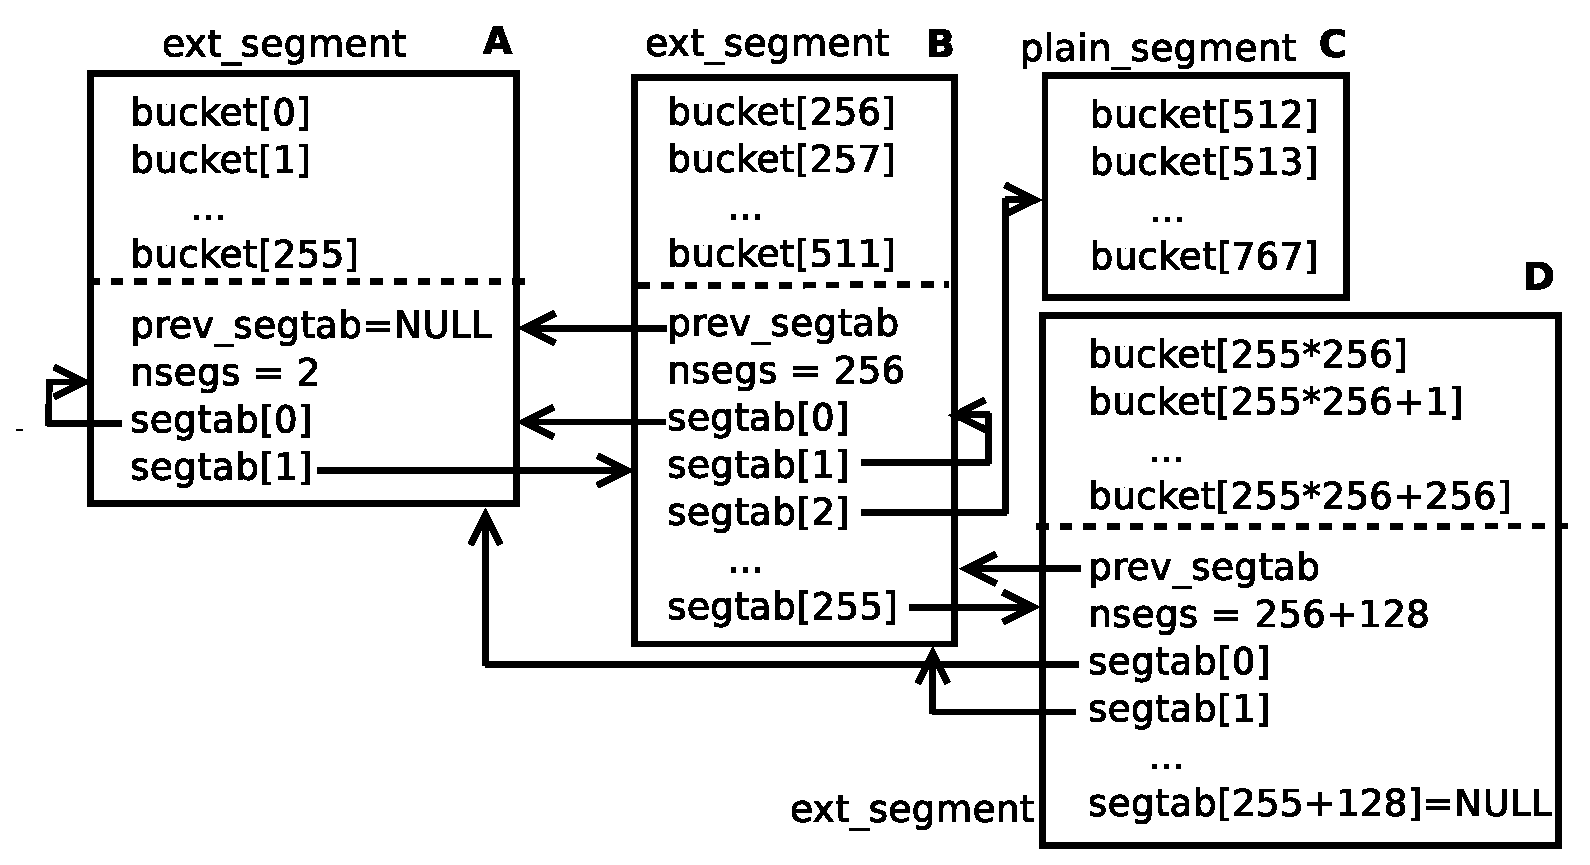
\includegraphics[width=1.0\textwidth]{hash_table_structure.eps}
  \caption{Hash table structure}
  \label{fig:hash_table_structure}
\end{figure}

\subsubsection{Expansion}

Expansion is triggered after table insertion when the total number of entries in the table exceeds a predefined value.
Currently this value is set so that if a uniform distribution of objects is assumed, each bucket has a chain length of 6.
Growing happens by splitting just one bucket, moving objects to the bucket after the one that is currently active.
The bucket to be split is the one obtained by dropping the newly active bucket's index most significant bit.
If the segment address of the new bucket corresponds to an index in the segment section that is currently not pointing to a bucket section, a new plain bucket section is allocated and the slot is now pointing to its first entry.
If this operation would assign a plain bucket section in the last slot of the segment section of the currently active extended segment, a new extended segment is allocated instead, with more slots in its segment section\footnote{
  The first extended segment has 2 slots in its segment section.
  The second extended segment has 256 slots in its segment section.
  Each next extended segment has 128 more slots in its segment section than the previous.
}.
After a new extended segment is allocated, all the pointers from the segment section of the old extended segment are copied into the low indices of the segment section of new extended segment.
This leads to duplication (the same plain bucket sections are accessible from multiple extended segment sections), but enables reaching the contents of a bucket by using the segment section of just the current extended segment.
The new extended segment does not immediately replace the old one as current.
The replacement happens when yet another segment must be allocated.
(This will be a plain segment, stored in the segment section of the new extended segment.)

\subsubsection{Shrinking}

Shrinking may happen after deletion, if the total number of entries falls below a predefined value.
Shrinking works in the reverse direction of growing:
The active bucket with the highest index is merged with its corresponding ``low'' bucket.

Shrinking might lead to the deallocation of a plain or extended bucket segment, if none of the buckets in it is active.
Once the first bucket not accessible through the previous extended segment is deallocated, the previous extended segment is restored as current extended segment.
This ``early replacement'' happens in order to avoid deallocating an extended segment while its segment table may still be used by other threads.
When the extended segment is later deallocated, the contents of all the buckets in the bucket section have been rehashed, seizing *all* locks, so there cannot exist any processes still executing code using the old extended segment pointer.

\subsubsection{Fine-grained Locking}

Protected and public hash tables support fine-grained locking if the option \verb|write_concurrency| is provided during creation.
In this case, apart from the main table lock, an additional array of locks is allocated during table creation and each lock ``protects'' a subset of the buckets.
The size of this lock array is currently defined at \emph{compile time} to 16.
(Therefore each lock protects those buckets whose index modulo 16 equals the lock's index.)


\subsubsection{Hash table types}     % section 2.1

With the underlying implementation being the same for all the types of hash tables, the specific type of the table introduces only minor differences in specific operations.

\paragraph{Set}

Insertion in tables of \verb|set| type should overwrite the existing value.
It should also fail if the insertion is performed with a insert\_new operation.

\paragraph{Bag, Duplicate Bag}

Special care should be taken to group together objects with the same key.

\subsection{Ordered Set table type}

The ordered set table type is implemented with an AVL tree.
An AVL tree was first described by G. M. Adelson-Velskii and E. M. Landis.
The current implementation uses one lock for the whole table.
The \verb|write_concurrency| option do not have any effect on tables of this table type.

\section{Concurrency Options} \label{sec:concurrency_options}

The options \verb|write_concurrency| and \verb|read_concurrency| are orthogonal.
The following table shows how the options affect the different table types:

\begin{center}
\begin{tabular}{l|p{5cm}|p{5cm}}
× & Hash based table types & \verb|ordered_set| table type \\ \hline
\verb|write_concurrency| & 
The buckets are divided between 16 locks. At most 16 write operations can be done concurrently. 
& Not affected\\
\verb|read_concurrency| & 
Different type of lock(s) optimized for frequent reads are used & 
A different type of lock optimized for frequent reads are used
\end{tabular}
\end{center} 

The concurrency options do not affect tables that are set to \verb|private| since they can only be accessed by one process.

Operations that modify several buckets always lock the whole table.
For example the insert operation may take a list of objects to insert.
If the parameter given to insert is a list, the whole table will be locket while the objects are inserted to make the operation atomic.

\section{Fixation}
\label{sec:fixation}

A process can call \texttt{ets:safe\_fixtable(Table, true $|$ false)} to put a fixation on a table implemented with a hash table (\verb|set|, \verb|bag| or \verb|duplicate_bag|).
When a table is fixed, a sequence of \verb|first/1| and \verb|next/2| calls are guaranteed to succeed and each object in the table will only be returned once, even if objects are removed or inserted during the traversal (keys for new objects inserted during the traversal may be returned by \verb|next/2|, depending on the internal ordering of the keys).
This high-level guarantee can be simplified into the following 2 low-level ones:

\begin{enumerate}
\item Keys will not totally disappear from the table.
  A key can thus be used as an iterator to find the next key in iteration sequence.
  Note however that this does not mean that (pointers to) table objects are guaranteed to be maintained while the table is fixated.
  A \verb|bag| or \verb|duplicate_bag| may actually remove objects as long as there is at least one object left in the table with the same key.
\item Objects will not be moved between buckets due to table grow/shrink.
  This will guarantee that iterations do not miss keys or get double-hits.
\end{enumerate}

\subsection{Implementation}

Fixation is monitored by a flag on the table itself and a mapping between PIDs and the identifiers of the tables that the respective process has fixated.
The fixation flag is checked before growing or shrinking a table to make sure that possible split or merges won't lead into duplicate appearance of objects in a traversal.
Objects on a fixed table are not deleted if there exist no other objects with the same key.
Instead objects are marked with an ``invalid\_hash'' flag (pseudo-deleted) and added to a list with objects that must be deleted after the fixation has been lifted.

The mapping of PIDs and TIDs is used to remove fixations when processes exit.

\section{Benchmark} \label{sec:benchmark}

A simple benchmark has been performed.
The purpose of the benchmark is to see how the \verb|write_concurrency| and \verb|read_concurrency| options affect the performance of different table types on a ``real'' problem.
The benchmark creates workers that all do \verb|lookup|s and \verb|insert|s on the same ETS table.
It was run on a computer with 64 cores (AMD Bulldozer Architecture).
It was run with all combinations of \verb|write_concurrency| and \verb|read_concurrency| together with the table types \verb|set| and \verb|ordered_set|.

\subsection{Benchmark Problem}
The benchmark program finds the minimum number of sort steps to sort an array, containing \emph{black} marks, \emph{white} marks and \emph{empty} positions.
As an example the sequence \verb|"ebbwe"| represents such an array, with \verb|e| marking \emph{empty} position, \verb|w| representing \emph{white} mark and \verb|b| representing \emph{black} mark.
Black marks can only move towards the right end of the array and white marks can only move towards the left end.
In one sort step a mark can:
\begin{itemize}
\item move one step in the array if the adjacent position in the direction of the movement is \emph{empty} or
\item move two steps in the array, if the adjacent position in the direction of the movement contains \emph{a mark} and the position after the adjacent position is \emph{empty}.
\end{itemize}
A sorted array has all white marks in the leftmost positions and all black marks in the rightmost positions.
Some input arrays are impossible to sort with the given constraints, e.g. \verb|"bbww"|.
If the input array can not be sorted the program shall return $-1$.
For example the minimum number of steps for \verb|"ebbwe"| is $5$.
The benchmark measures time needed to return the result for the arrays \verb|"bebebbeeeewwwbw"| and \verb|"bebebeeewewewewwe"|.

\subsection{Implementation}
The Erlang program that solves the benchmark problem is available on www.github.com\footnote{http://github.com/kjellwinblad/ets\_impl\_project/blob/master/benchmark/multi\_4.erl}.
The program explores the possible solutions using breadth first search.
Explored configurations are saved in an ETS table to avoid repeating work.

The program has one coordinator process and a number of worker processes.
At a specific level in the search tree, the coordinator divides the configurations that need to be explored in the next level evenly and sends them to the workers.
The workers send a message to the coordinator if a solution is found.
If a worker gets a configuration that is not a solution, the configuration is expanded by generating all possible configurations that can be created by performing one sort step.

Directly after a configuration is generated, it is checked whether the configuration already exists in the ETS table cache with the \verb|ets:member| function.
If it already exists, it is thrown away because the configuration has already been visited.
Otherwise, the configuration is inserted in the ETS table with the \verb|ets:insert_new| operation.
The return value of \verb|ets:insert_new| is checked to make sure that the configuration has not been inserted by another process between the call to \verb|ets:member| and \verb|ets:insert_new|.
The Erlang code that is interacting with the ETS table cache in the workers can be seen in Listing~\ref{li_erlang_ets_interaction}. 

\lstset{basicstyle=\ttfamily, keywordstyle=\bfseries, language=erlang, caption=Worker code that is interacting with ETS, label=li_erlang_ets_interaction}
\begin{lstlisting}[float=htb]
IsFound = ets:member(Cache, MoveArray),
case IsFound of
  false ->
    Inserted = ets:insert_new(Cache, {MoveArray}),
    case Inserted of
      true ->
        [MoveArray|all_next_step_arrays(Array, CurrentPos + 1, Cache)];
      false ->
        all_next_step_arrays(Array, CurrentPos + 1, Cache)
    end;
  true ->
    all_next_step_arrays(Array, CurrentPos + 1, Cache)
end
\end{lstlisting}

A worker sends back all the configurations that need to be explored in the next level to the coordinator, when it has processed all given configurations on the current level.

\subsection{Results} 

The results of the benchmark can be seen in Figure~\ref{fig:benchmark_results}.
The filled straight line labeled \emph{serial} is the performance of a serial version of the benchmark program.
The serial version can also be found on www.github.com\footnote{http://github.com/kjellwinblad/ets\_impl\_project/blob/master/benchmark/single\_1.erl}.
The graphs with ``set'' in the label show the benchmark times for the table type \verb|set|.
The graphs with ``ordset'' in the label show the benchmark times for the table type \verb|ordered_set|.
A ``w'' in the label means that the table has \verb|write_concurrency| enabled and an ``r'' in the label means that the table has \verb|read_concurrency| enabled.

\begin{figure}[htb]
\centering
\includegraphics[width=1.0\textwidth]{benchmark.eps}
\caption{Benchmark Results}
\label{fig:benchmark_results}
\end{figure}

The table type \verb|set| with \verb|write_concurrency| enabled seems to give similar performance both with and without \verb|read_concurrency| enabled.
All other configurations have similar performance.
The \verb|write_concurrency| option does not affect the table type \verb|ordered_set| so the graphs with  \verb|write_concurrency| enabled together with \verb|ordered_set| are not included.
The \verb|ordered_set| table type should theoretically have more expensive \verb|lookup| and \verb|insert| operations compared to the \verb|set| table type.
This does not seem to have any significant effect on this benchmark.

It is clear that \verb|set| table type with \verb|write_concurrency| enable scale best for this benchmark.
This is not surprising since \verb|set| together with \verb|write_concurrency| allow processes to do other operations on the table, concurrently during write operations. 

\section{Scalable ETS Suggestions}

The benchmark described in Section~\ref{sec:benchmark}, shows that fine grained locking (provided by the \verb|write_concurrency| option) can be very important for scalability.
The number of locks used when fine grained locking is enabled is hard-coded to 16 in the current implementation.
It is tempting to make the locking even more fine grained, since it could possibly make ETS more scalable.
However, it might increase processor cache misses since more locks make use of more memory.
The benchmark described in Section~\ref{sec:benchmark} has also been run with versions of the runtime environment with the number of locks set to 32 and 64.
This change did not seem to have any significant effect on the performance of the benchmark program.
There might be other bottlenecks in this particular benchmark that are more important.
It would be interesting to look more deeply into how the number of locks affects the performance of other benchmarks.

The benchmarks of Judy-array based ETS table implementations that are described by Fritchie suggests that there are other table implementations that are significantly faster than the current ones for some use cases~\cite{ScottEtsJudy}.
Fritchie did not discuss how to make the Judy-array based ETS table implementation concurrent.
Prokopec, Bagwell and Odersky have described a ``lock-free'' concurrent data type called CTrie~\cite{ProkopecCTrie} which is similar to the ETS table implementation suggested by Fritchie.
Benchmarks indicate that CTries scale well for insert operations~\cite{ProkopecCTrie}.
Using a CTrie to implement ETS tables could potentially provide better scalability than the current implementation for some use cases.

The current ETS table implementation has no good support for use cases when more than one table operation need to be performed atomically.
The only practical way to support that use case with the current ETS implementation is to serialize all access to the ETS table or ETS tables involved.
The serialization can be done by using a process as a proxy to the ETS table.
Transactional support for ETS tables as suggested by Nyblom~\cite{PatrikErlangTrans} could be a way to support this use case in a much more scalable way.

In the current implementation of ETS, all terms that are inserted or fetched from an ETS table are copied from or to the ETS table.
This might be expensive both in respect to time and memory if many processes access the same objects in the table.
An alternative would be to use references for terms that are stored in ETS tables.
The Erlang runtime already uses references for values of the binary data type.
Therefore, it might be possible to reuse some existing components in the Erlang runtime system, to implement references for terms stored in the ETS tables with some potential performance benefits.

The current \verb|ordered_set| table type uses only one lock for the whole data structure.
There exist implementations of binary trees that scale well and that have support for efficient traversal of the tree.
Bronson, Casper, Chafi and Olukotun have described a relaxed AVL-tree data-structure with STM inspired methods for thread safety~\cite{BronsonPracTree}.
This implementation could give much better scalability on a multi-core computer than the current \verb|ordered_set| implementation.

Furthermore, there are many more concurrent implementations of lookup tables that could be used in ETS and potentially provide better scalability.
It could be interesting to do a more in-depth study of the implementation that are in use today.
For example \verb|ConcurrentHashMap| in the Java library does not require any locks for lookup operations \cite{BrianConcHashMap}.


\bibliographystyle{plain}
\bibliography{report}

\end{document}
